\documentclass[10pt,a4paper,twocolumn,twoside]{article}
\usepackage[utf8]{inputenc}
\usepackage[T1]{fontenc}
\usepackage[catalan]{babel}
\usepackage{multicol}
\usepackage{graphicx}
\usepackage{fancyhdr}
\usepackage{times}
\usepackage{titlesec}
\usepackage{multirow}
\usepackage{lettrine}
\usepackage[backend=biber, style=numeric, sorting=none]{biblatex}
\usepackage[top=2cm, bottom=1.5cm, left=2cm, right=2cm]{geometry}
\usepackage{url}
\usepackage{float}
\usepackage[figurename=Fig.,tablename=TAULA]{caption}
\usepackage{booktabs}
\usepackage{subcaption}
\usepackage{amsmath}
\usepackage{amssymb}
\usepackage{xcolor}
\usepackage{colortbl}
% \usepackage{parskip}
\addbibresource{references.bib}
\captionsetup[table]{textfont=sc}
\usepackage[hidelinks]{hyperref}
\usepackage{tikz}
\usetikzlibrary{arrows.meta,positioning,calc}

\author{\LARGE\sffamily David Morillo Massagué}
\title{\Huge{\sffamily Predicció de Metàstasis en Histopatologia en Càncer Colorrectal usant

Graph Attention Networks}}

\date{}

\newcommand\blfootnote[1]{%
  \begingroup
  \renewcommand\thefootnote{}\footnote{#1}%
  \addtocounter{footnote}{-1}%
  \endgroup
}

\titleformat{\section}
{\large\sffamily\scshape\bfseries}
{\textbf{\thesection}}{1em}{}

\begin{document}

\fancyhead[LO]{\scriptsize David Morillo Massagué: Predicció de Metàstasi en Histopatologia usant GATs}
\fancyhead[RO]{\thepage} \fancyhead[LE]{\thepage}
\fancyhead[RE]{\scriptsize EE/UAB TFG DADES: Predicció de Metàstasi en Histopatologia usant GATs}

\fancyfoot[CO,CE]{}

\fancypagestyle{primerapagina}
{
   \fancyhf{}
   \fancyhead[L]{\scriptsize TFG EN ENGINYERIA DADES, ESCOLA D'ENGINYERIA (EE), UNIVERSITAT AUTÒNOMA DE BARCELONA (UAB)}
   \fancyfoot[C]{\scriptsize Juliol de 2026, Escola d'Enginyeria (UAB)}
}

\renewcommand{\headrulewidth}{0pt}
\renewcommand{\footrulewidth}{0pt}
\pagestyle{fancy}

\twocolumn[\begin{@twocolumnfalse}

\maketitle

\thispagestyle{primerapagina}

\begin{center}
\parbox{0.915\textwidth}
{\sffamily
\textbf{Resum--}
Es presenta un sistema de classificació N0/N1 per a la detecció de metàstasi en ganglis limfàtics
en càncer colorrectal pT1 a partir de \textit{Whole Slide Images}. El teixit es representa com un
\textbf{graf espacial} construït per triangulació de Delaunay sobre les coordenades dels \textit{patches},
de manera que es preserva la topologia real del teixit, a diferència d'enfocaments basats en similitud de
característiques. Cada node és un \textit{patch} de 2048$\times$2048 px representat per l'embedding
CLS (1.536 dim.) del model UNI2. Es comparen dues arquitectures configurables: un GAT de referència
amb \textit{readout} pla (mean, max, mean\_max o attention) i un GAT amb \textbf{DiffPool jeràrquic}
intercalat ($N \to \cdots \to K_L$ super-nodes, nombre de blocs $L_{\text{DP}}$ optimitzat) per
obtenir representacions a múltiples escales. El diagnòstic per pacient s'obté per
agregació MIL sobre les seccions. La cerca d'hiperparàmetres combina dos estudis Optuna
TPE aïllats per arquitectura amb una re-avaluació estricta (5-fold CV + retrain final
90/10) de les millors configuracions obtingudes. \textbf{El millor model és un GAT
Baseline} (attention pooling, MIL=mean, $h=256$, $H=4$, dropout $0{,}3$,
$\lambda_{\text{wd}}=10^{-4}$) que obté AUC test $=0{,}875$, sensibilitat $100\%$ i
especificitat $57{,}5\%$ al llindar derivat del val set, detectant els 16 casos N1 del
conjunt de test ($n=56$ pacients; 367 pacients efectius en total).
\\
\\
\textbf{Paraules clau-- } Càncer colorrectal pT1, Histopatologia digital, Graph Attention Networks,
DiffPool jeràrquic, Graf espacial de Delaunay, MIL, Desbalanceig de classes.\\
\\
\bigskip
\\
\textbf{Abstract--}
We present an N0/N1 classification system for lymph node metastasis prediction in pT1 colorectal
cancer from Whole Slide Images. Tissue is represented as a \textbf{spatial graph} built by Delaunay
triangulation over patch coordinates, preserving the real spatial topology of the tissue, unlike
feature-similarity graph approaches. Each node is a 2048$\times$2048 px patch represented by a
1,536-dimensional CLS embedding from the UNI2 model. Two configurable architectures are compared: a
\textbf{GAT baseline} with flat readout (mean, max, mean\_max or attention) and a \textbf{GAT+DiffPool} model
with $L_{\text{DP}}$ DiffPool blocks interleaved between GAT layers ($N \to \cdots \to K_L$ super-nodes) for
multi-scale representations. Patient-level diagnosis is obtained via MIL aggregation over
histological sections. Hyperparameter search combines two isolated Optuna TPE studies
(one per architecture) with a strict re-evaluation (5-fold CV + 90/10 retraining) of
the best configurations. \textbf{The best model is a GAT Baseline} (attention pooling,
MIL=mean, $h=256$, $H=4$, dropout $0.3$, $\lambda_{\text{wd}}=10^{-4}$) achieving test
AUC $=0.875$, sensitivity $100\%$ and specificity $57.5\%$ at the validation-derived
threshold, detecting all 16 N1 cases of the test set ($n=56$ patients; 367 effective
patients overall).
\\
\\
\textbf{Keywords-- } pT1 colorectal cancer, Digital histopathology, Graph Attention Networks,
Hierarchical DiffPool, Spatial Delaunay graph, Multiple Instance Learning, Class imbalance.\\
}

\bigskip

{\vrule depth 0pt height 0.5pt width 4cm\hspace{7.5pt}%
\raisebox{-3.5pt}{\fontfamily{pzd}\fontencoding{U}\fontseries{m}\fontshape{n}\fontsize{11}{12}\selectfont\char70}%
\hspace{7.5pt}\vrule depth 0pt height 0.5pt width 4cm\relax}

\end{center}

\bigskip
\end{@twocolumnfalse}]

\blfootnote{$\bullet$ E-mail de contacte: David.MorilloMa@autonoma.cat}
\blfootnote{$\bullet$ Treball tutoritzat per: Debora Gil Resina (DCC)} \blfootnote{$\bullet$ Curs 2025/26}

\section{Introducció}

\lettrine[lines=3]{E}{l} càncer colorrectal (CCR) és un dels reptes de salut pública més greus del nostre
entorn. A Espanya, la SEOM preveu per al 2026 més de \textbf{44.132} nous casos anuals, fet que el converteix en el tumor
més freqüent i en la segona causa de mort per càncer, amb 14.629 defuncions \cite{seom2026}.

El carcinoma pT1 és especialment complex: el tumor ha envaït la submucosa però no la muscular pròpia, i el risc de
metàstasi als ganglis limfàtics oscil·la entre el \textbf{2\%} i el \textbf{23\%} depenent de la profunditat
d'invasió \cite{ParcSalutMar2013}. % [NEW: comparison]
Quan hi ha criteris de mal pronòstic (\textbf{invasió submucosa $\boldsymbol{\geq\!1000\,\mu}$m,
invasió vascular o limfàtica, histologia indiferenciada, \textit{tumor budding} de
grau~$\geq\!2$ o marge vertical positiu} \cite{jsccr2019,dawson2024budding}), el risc puja
al voltant del $10\%$, fet que porta les guies clíniques (JSCCR \cite{jsccr2019}, NCCN i
ESMO \cite{esge2022}) a recomanar cirurgia radical addicional. Com que la majoria de tumors
pT1 no desenvolupa LNM real, s'estima que \textbf{més del $80\%$} d'aquestes cirurgies són
innecessàries \cite{zaffalon2023,MartinezDeJuan2024}.

La histopatologia digital, mitjançant les \textit{Whole Slide Images} (WSI), permet aplicar
tècniques avançades de visió per computador. En concret, les \textit{Graph Attention Networks}
(GAT) \cite{veličković2018graphattentionnetworks} permeten modelar el teixit com una estructura
espacial. Una decisió clau en la construcció del graf és el criteri de les arestes: alguns
treballs les basen en la \textit{similitud de característiques} entre \textit{patches}; aquest
treball opta per la \textbf{proximitat espacial} (triangulació de Delaunay sobre coordenades
WSI), preservant la topologia real del teixit. El projecte, desenvolupat al grup IAM del CVC
(iam.cvc.uab.es) sota la supervisió de la Dra.\ Debora Gil, compara un GAT de referència
amb \textit{readout} pla contra un model amb \textit{pooling} jeràrquic (DiffPool) intercalat,
i proposa diferents estratègies d'agregació MIL per al diagnòstic per pacient.

Dues raons justifiquen aquest treball. Des del punt de vista clínic, els sistemes d'IA poden
detectar patrons morfològics subtils de manera consistent i ajudar a reduir cirurgies
innecessàries. Des del punt de vista tècnic, combinar xarxes d'atenció sobre grafs amb
aprenentatge profund sobre WSI és just la intersecció entre teoria de grafs i deep learning
que vull explorar dins de l'Enginyeria de Dades.

\section{Objectius}

\begin{itemize}
    \item Construir un \textit{pipeline} complet de classificació N0/N1 sobre WSI reals a partir
    d'embeddings CLS del model UNI2, basat en \textbf{grafs espacials} (triangulació de Delaunay
    sobre coordenades del teixit).
    \item \textbf{Comparar un GAT de referència} amb \textit{readout} pla contra un model amb
    \textbf{DiffPool jeràrquic} intercalat entre capes GAT, avaluant si la reducció
    progressiva del graf aporta millor representació multi-escala.
    \item Implementar i comparar estratègies d'agregació MIL a nivell de pacient per integrar
    les prediccions de múltiples seccions histològiques.
\end{itemize}

\section{Estat de l'Art}

\subsection{Classificació de WSI amb MIL}

Les \textit{Whole Slide Images} tenen resolucions de fins a $150\,000 \times 150\,000$
píxels i no es poden processar directament amb xarxes convencionals. L'enfocament habitual
és dividir la làmina en \textit{patches} petits i treballar amb \textit{Multiple Instance
Learning} (MIL), on el model ha d'inferir l'etiqueta global a partir de fragments sense
etiqueta individual. Ilse et al.~\cite{ilse2018attentionbaseddeepmultipleinstance} van
proposar l'agregació per atenció (\textit{attention-based MIL}), que aprèn quins
\textit{patches} són més rellevants per al diagnòstic. Lu et al.~\cite{lu2020dataefficientweaklysupervised}
van aplicar aquest mètode a conjunts de dades clínics reals (CLAM), i Li et
al.~\cite{li2021dualstreammultipleinstancelearning} van proposar DSMIL, que combina dues
branques, a nivell de \textit{patch} i de làmina, amb aprenentatge contrastiu. La
predicció de metàstasi ganglionar a partir d'histopatologia s'ha estudiat en altres càncers:
Muti et al.~\cite{muti2023deep} mostren que és possible predir l'estat N0/N1 a partir de
làmines de càncer gàstric, amb resultats prometedors.

\subsection{Grafs i GNN en Patologia Digital}

Les \textit{Graph Neural Networks} permeten tractar el teixit com una estructura on les
regions estan connectades segons la seva proximitat, capturant relacions espacials que les
CNN no modelen directament. Jaume et al.~\cite{jaume2021histocartographytoolkitgraphanalytics}
van presentar HistoCartography, un entorn de treball per a l'anàlisi de grafs en patologia
digital, amb resultats que mostren millores respecte de les CNN en classificació de
biòpsies. Les GAT~\cite{veličković2018graphattentionnetworks} afegeixen un mecanisme
d'atenció que permet al model ponderar cada veí de manera diferent, cosa especialment útil
en histopatologia on no totes les regions del teixit aporten la mateixa informació. Pel que
fa al \textit{pooling} en grafs, Grattarola et al.~\cite{Grattarola_2024} revisen els
principals mètodes existents, entre ells DiffPool~\cite{ying2019hierarchicalgraphrepresentationlearning},
que agrupa nodes en super-nodes de manera progressiva.

\subsection{Models de Fundació per a Histopatologia}

En els darrers anys han aparegut \textit{foundation models} preentrenats específicament
sobre dades de patologia, que generen embeddings molt més informatius que les CNNs
genèriques. UNI2~\cite{chen2024uni2} és un \textit{vision transformer} entrenat sobre
més de 100 milions de \textit{patches} de 20 tipus de teixit, amb bons resultats en
nombroses tasques de classificació histopatològica. CONCH~\cite{lu2024conch} és un model
similar que incorpora a més alineament entre imatge i text. En aquest projecte s'utilitzen
els embeddings de UNI2 com a vector de característiques de cada node, ja que estan
preentrenats en el mateix domini i capturen informació morfològica rellevant.

% [NEW: comparison]
\subsection{Guies Clíniques i Models Predictius per a pT1 CRC}
\label{sec:guidelines-sota}

Les guies clíniques de referència (JSCCR \cite{jsccr2019}, NCCN i
ESMO \cite{esge2022}) recomanen cirurgia addicional quan el pacient
presenta un o més dels criteris de risc histopatològics esmentats a la
Introducció. Malgrat la seva sensibilitat elevada, la seva especificitat
és baixa: en un estudi comparatiu sobre $560$ pacients
\cite{tanino2024comparative}, les AUC reportades són $0{,}596$ (JSCCR),
$0{,}749$ (NCCN) i $0{,}743$ (ESMO), amb especificitats del $19\%$, $52\%$
i $50\%$ respectivament, la qual cosa implica que més del $80\%$ dels
pacients operats no tenien LNM real \cite{tanino2024comparative,zaffalon2023}.

Paral·lelament, Piao et al.~\cite{piao2023ai} van proposar un model
d'IA sobre variables clinicopatológiques ($n\!=\!546$ entrenament,
$n\!=\!105$ test) basat en gradient boosting (\textit{LightGBM}),
obtenint sensibilitat del $100\%$, especificitat del $85{,}8\%$, AUC de
$0{,}960$ i \textit{balanced accuracy} del $92{,}9\%$; la taxa de
pacients classificats com a alt risc es va reduir del $83{,}8\%$ (JSCCR)
al $20{,}9\%$. Dawson et al.~\cite{dawson2024budding} van proposar
l'IBC Score, una puntuació ponderada sobre invasió limfovascular, grau de
\textit{tumor budding}, profunditat d'invasió i grau tumoral,
que obté AUC de $0{,}68$ sobre $565$ pacients. A diferència d'aquests
treballs, aquest TFG fa la predicció exclusivament a partir de la
\textbf{imatge histopatològica} (WSI), sense variables clíniques
estructurades ni puntuació manual d'un patòleg.

\subsection{Treball Previ al CVC sobre pT1 CRC}

Aquest treball s'integra dins una línia de recerca del grup IAM del CVC. Martí et
al.~\cite{ddd.uab.cat:317556} van comparar CNNs, ViTs i GNNs sobre el mateix conjunt
pT1 CRC per a la classificació de \textit{patches} individuals, amb millor AUC
($0{,}954 \pm 0{,}077$) per una arquitectura híbrida ViT+NN. Aquell treball, però,
opera a nivell de \textit{patch} i no té en compte la topologia espacial del teixit
ni el diagnòstic per pacient. Aquest TFG parteix dels embeddings CLS del model UNI2
per construir grafs espacials de les seccions i aborda el problema des d'una
perspectiva MIL per pacient.

\section{Dades i Preprocessament}

Aquest projecte es realitza en col·laboració amb un equip de la UAB que cobreix des de la recollida de dades fins
a la creació d'autoencoders per a l'extracció de característiques.

\subsection{Imatges de Gran Format (WSI)}

Les dades originals consisteixen en imatges de làmines senceres (WSI) obtingudes amb escàners d'alta resolució i
tintades amb hematoxilina-eosina, emmagatzemades en format MIRAX (\textit{.mrxs}). Les dimensions oscil·len entre
els 30.000 i els 150.000 píxels per costat, amb una quantitat significativa d'espai buit o artefactes que
requereixen tractament previ.

El conjunt de dades efectiu comprèn \textbf{1.607 grafs} (un per secció histològica), provinents de
\textbf{367 pacients} distribuits de forma desequilibrada entre les dues classes
(Taula~\ref{tab:dataset}). D'un total de 606 pacients a la base de dades clínica, 236 es descarten
per diagnòstic indeterminat (NX), i dels 370 restants amb diagnòstic vàlid, 3 no disposen
d'embeddings UNI2 generats, deixant 367 pacients usables. Les mostres es divideixen en un \textbf{pool d'entrenament+validació (85\%)} i un
\textbf{conjunt de test fix (15\%)}, ambdós estratificats a nivell de pacient. Dins del pool s'aplica
validació creuada 5-fold per a la cerca d'hiperparàmetres (Secció~\ref{sec:training-scheme}).

\begin{table*}[t]
\centering
\caption{Composició del dataset efectiu per partició (26 hospitals).
Els grafs corresponen a seccions histològiques individuals (un per secció). El pool (85\%)
s'utilitza per a la cerca d'hiperparàmetres amb validació creuada 5-fold; el test (15\%)
es reserva per a l'avaluació final.}
\label{tab:dataset}
\small
\begin{tabular}{lrrr|rrr}
\toprule
 & \multicolumn{3}{c|}{\textbf{Pacients}} & \multicolumn{3}{c}{\textbf{Grafs (seccions)}} \\
\textbf{Partició} & \textbf{N0} & \textbf{N1} & \textbf{Total} & \textbf{N0} & \textbf{N1} & \textbf{Total} \\
\midrule
Pool (train+val CV) & 224 &  87 & 311 & 1\,133 & 219 & 1\,352 \\
Test                &  40 &  16 &  56 &   212  &  43 &   255  \\
\midrule
Total & 264 & 103 & 367 & 1\,345 & 262 & 1\,607 \\
\bottomrule
\end{tabular}
\end{table*}

\subsection{Anotacions i Màscares de Segmentació}
\label{sec:anotacions-masques}

La Dra.\ Eva Musulén, patòloga especialitzada, ha realitzat les anotacions manualment amb el programari
\textit{Labelme}. Aquestes identifiquen tres categories d'afectació:

\begin{itemize}
    \item \textbf{Infiltració:} teixit anormal que envaeix zones no corresponents.
    \item \textbf{Displàsia:} cèl·lules anormals que poden convertir-se en canceroses.
    \item \textbf{Infiltració + Displàsia:} usat en casos de dubte diagnòstic.
\end{itemize}

A partir d'aquestes s'obtenen màscares de segmentació codificades per color: vermell (infiltració), blau
(displàsia) i verd clar (combinada).

\begin{figure}[h]
    \centering
    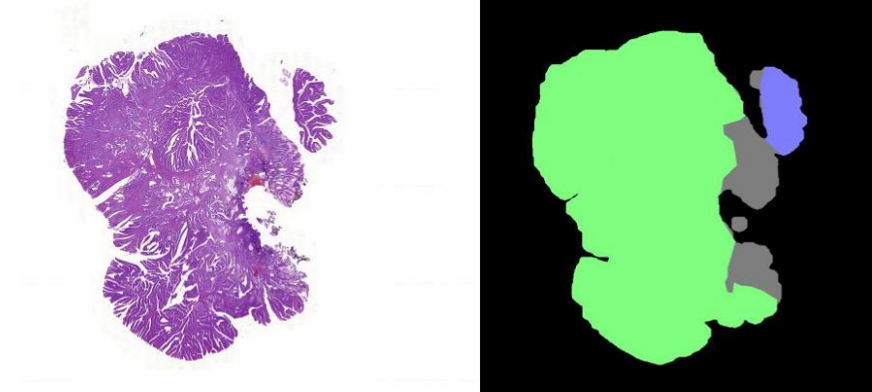
\includegraphics[width=0.45\textwidth]{img/mascara.png}
    \caption{Exemple de WSI i la seva corresponent màscara de segmentació.}
    \label{fig-mask}
\end{figure}

\subsection{Extracció de Patches i Embeddings CLS}

S'aplica una finestra lliscant (\textit{sliding window}) sense solapament per dividir cada làmina en
\textit{patches} de $2048 \times 2048$ píxels a resolució completa (nivell 0). El model de fundació
\textbf{UNI2}~\cite{chen2024uni2} processa cada \textit{patch} individualment i extreu el token
\textit{CLS} de la seva sortida, obtenint un vector de \textbf{1.536 dimensions} que condensa la
informació morfològica i textural del patch.

\textbf{Filtratge dels \textit{patches}.} L'única selecció es fa \textbf{abans del càlcul de
l'embedding}, durant la pròpia extracció des del WSI: per cada finestra, es comprova el
\textbf{percentatge de teixit} a la corresponent regió de la \textbf{màscara binària anotada}
(\S\ref{sec:anotacions-masques}); les finestres sense cap píxel de teixit
(\textit{tissue\_percentage}~$= 0$) o que cauen fora d'una component connexa anotada vàlida
es descarten i \textbf{no s'extreuen ni passen per UNI2}. La resta sí es guarden al disc i
generen un node del graf. Estadístiques de qualitat com la \textit{borrositat}, la \textit{proporció
de píxels blancs} o la \textit{desviació estàndard} de cada \textit{patch} es calculen i s'emmagatzemen
com a metadades, però \textbf{no} s'usen per filtrar.

\section{Construcció del Graf}

\subsection{Model de dades: dimensions i estructures}
\label{sec:model-dades}

Formalment, cada secció histològica es representa com un graf
$\mathcal{G} = (\mathbf{X},\,\mathbf{A})$ on:
\begin{itemize}
  \item $\mathbf{X} \in \mathbb{R}^{N \times 1536}$ és la matriu de característiques dels $N$ nodes
        (\textit{patches}).
  \item $\mathbf{A} \in \{0,1\}^{N \times N}$ és la matriu d'adjacència construïda per triangulació
        de Delaunay i posterior poda d'arestes llargues.
\end{itemize}

Dues estratègies de \textit{pooling} transformen la seqüència de grafs en un vector global que
alimenta el capçal MLP per produir $P(\text{N1})$:
\begin{itemize}
  \item \textbf{Pla (\textit{readout}).} Operació global sobre les sortides de la darrera capa GAT,
  sense reduir el graf: \textit{mean}, \textit{max}, \textit{sum}, \textit{mean\_max} (concatenació
  de mean i max) o \textit{attention} (pes escalar aprenible per node). Estratègia configurable.
  \item \textbf{Jeràrquic (DiffPool intercalat).} Un nombre configurable $L_{\text{DP}} \in \{1,2,3\}$
  de blocs DiffPool s'intercalen entre capes GAT, col·lapsant progressivament el graf de $N$ nodes
  fins a $K_{L_{\text{DP}}}$ super-nodes. Cada nivell aprèn una matriu d'assignació suau i produeix
  un nou graf de menor grandària.
\end{itemize}

\textbf{Estratègia adoptada: un graf per secció.} Cada secció genera un graf independent;
les $S$ seccions d'un pacient es processen per separat i les probabilitats
$\{P(\text{N1}_i)\}_{i=1}^{S}$ s'agreguen via MIL (Secció~\ref{sec:mil}).
Com a alternativa es va explorar un \textit{mega-graf} per pacient (bloc-diagonal de totes les seccions
sense arestes entre elles), però va donar resultats inferiors (veure Secció~\ref{sec:main-effects}),
probablement per forçar un únic \textit{pooling} global sobre teixits físicament inconnexos.
\subsection{Connectivitat per triangulació de Delaunay}

Una connectivitat fixa de reixeta no és adequada perquè la màscara exclou regions de fons i trenca la
simetria de la quadrícula. Per aquest motiu, s'aplica una \textbf{triangulació de Delaunay} sobre els
nodes restants, que s'adapta a distribucions irregulars de forma natural. A continuació, s'eliminen les
arestes que travessen píxels de valor zero a la màscara, evitant connexions entre regions separades per
espai buit. Finalment, s'aplica un criteri de distància màxima: s'eliminen les arestes que superen el
doble de la longitud mitjana del conjunt. La figura~\ref{fig:preprocess} mostra el resultat del procés: les arestes eliminades pel filtre de màscara apareixen en vermell.

\textbf{Secció $\equiv$ component connexa.} La definició de \textit{secció} prové del pipeline
d'extracció de patches, que aplica \texttt{cv2.connectedComponentsWithStats} sobre la màscara
binària de teixit. Per construcció, una secció correspon a \textbf{una component connexa de la
màscara}: les illes de teixit no adjacents són tractades com a seccions independents (un graf per
illa). Empíricament, sobre les 1.607 seccions del dataset, el 100\% generen un graf Delaunay
d'una sola component, fet coherent amb aquesta definició.

\begin{figure*}[h]
    \centering
    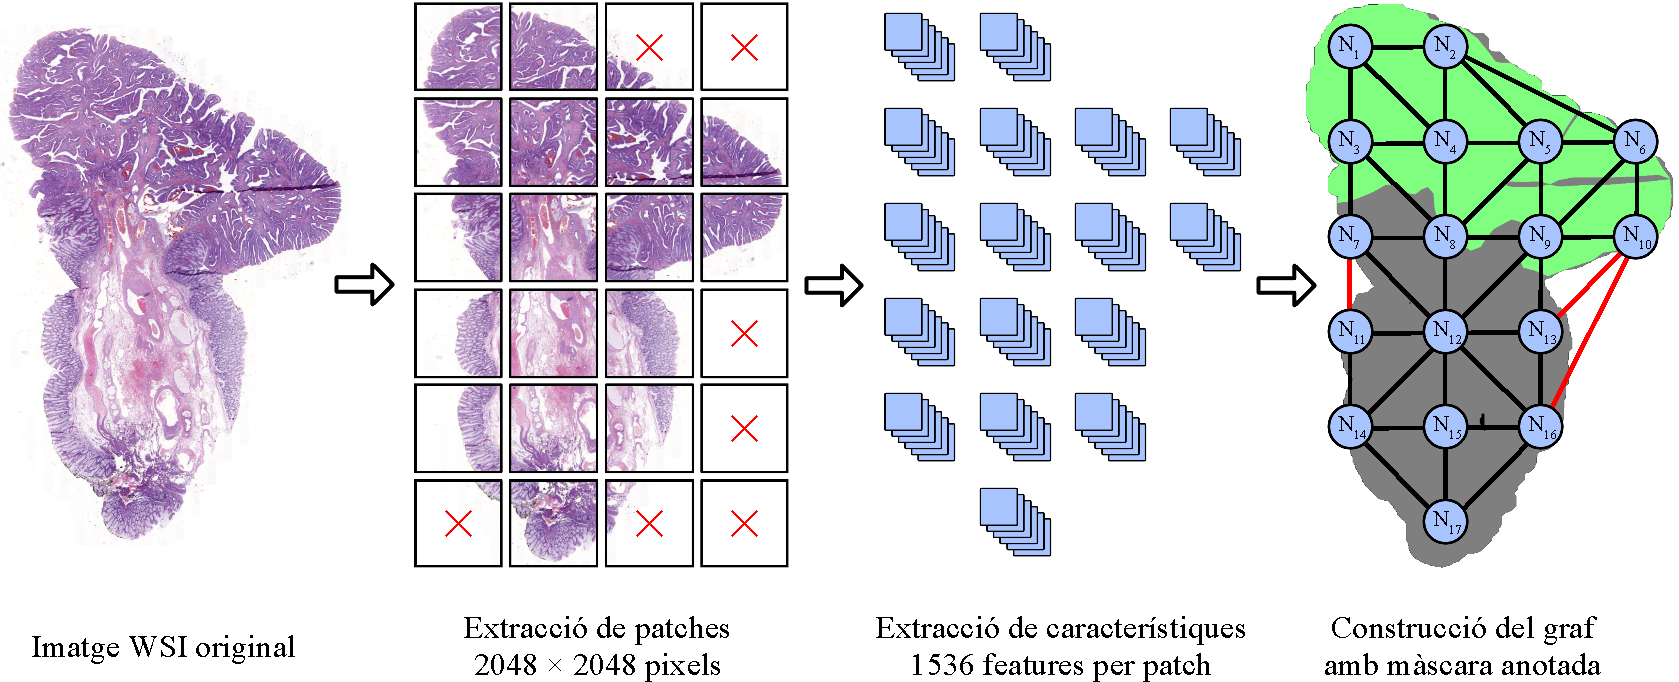
\includegraphics[width=0.8\textwidth]{img/preprocess.pdf}
    \caption{Etapes del preprocessament per a la construcció del graf. D'esquerra a dreta:
    WSI original $\to$ extracció de \textit{patches} de $2048{\times}2048$ px per finestra lliscant + filtratge
    $\to$ extracció de l'embedding CLS de 1.536 dimensions per UNI2 (un vector per \textit{patch})
    $\to$ construcció del graf de Delaunay sobre la màscara anotada, on les arestes en vermell han
    estat eliminades pel filtre de màscara}
    \label{fig:preprocess}
\end{figure*}

\section{Arquitectura del Model}

\subsection{Visió general del pipeline}
\label{sec:pipeline-overview}

El sistema encadena set mòduls: (i) lectura del WSI, (ii) extracció de \textit{patches}
2048$\times$2048, (iii) càlcul de l'embedding CLS de 1.536 dimensions amb el model
\textit{foundation} UNI2, (iv) construcció del graf de Delaunay per secció amb poda
d'arestes llargues, (v) propagació amb $L$ capes GAT i \textit{pooling} (pla o jeràrquic
amb DiffPool), (vi) agregació MIL inter-secció per pacient, i (vii) decisió mitjançant un
llindar $t^*$ derivat del \textit{validation set}. Cada mòdul configurable té eixos
optimitzats per la cerca bayesiana (vegeu Annex \ref{app:pipeline-full} per al diagrama
detallat amb hiperparàmetres associats a cada bloc).

Les seccions següents descriuen el model (GAT, pooling pla i jeràrquic), l'agregació MIL
i el procediment d'entrenament.

\subsection{GATClassifier}

El model implementat, \texttt{GATClassifier}, és un classificador de grafs que alterna capes
\textbf{Graph Attention Network} (\texttt{GATConv}~\cite{veličković2018graphattentionnetworks,fey2019fastgraphrepresentationlearning})
amb capes de \textit{pooling} jeràrquic per a la classificació binària N0/N1. L'arquitectura és
completament parametritzable: el nombre de capes GAT, el nombre de blocs DiffPool intercalats i la
dimensió oculta es trien com a hiperparàmetres. Quan s'utilitza DiffPool, cada bloc inserit entre
capes GAT redueix el graf de $N_\ell$ nodes a $K_\ell$ super-nodes:
$(\mathbf{X}^{(0)}, \mathbf{A}^{(0)}) \xrightarrow{\text{GAT+Pool}} \cdots \xrightarrow{\text{GAT+readout}} \mathbf{z}$.
Tot el model s'entrena de forma \textbf{end-to-end}: un únic pas de retropropagació propaga els
gradients des del capçal MLP fins a les primeres capes GAT. La Figura~\ref{fig-diffpool} mostra
la comparació visual de les dues arquitectures.

\textbf{Mecanisme d'atenció.} A diferència de les xarxes convolucionals clàssiques sobre grafs que tracten
tots els veïns d'un node de forma uniforme, GAT aprèn a assignar pesos d'importància diferenciats a cada
veí. Donada la representació $\mathbf{h}_i$ del node $i$, per a cada parella de nodes
veïns $(i, j)$ es calcula un coeficient d'atenció:
\begin{equation*}
  e_{ij} = \text{LeakyReLU}\!\left(\mathbf{a}^{\top}[\mathbf{W}\mathbf{h}_i \,\|\, \mathbf{W}\mathbf{h}_j]\right)
\end{equation*}
on $\mathbf{W}$ és una transformació lineal aprenible, $\|$ la concatenació i $\mathbf{a}$ un vector
aprenible. Els coeficients es normalitzen amb \textit{softmax} sobre tots els veïns:
\begin{equation*}
  \alpha_{ij} = \frac{\exp(e_{ij})}{\sum_{k \in \mathcal{N}(i)} \exp(e_{ik})}
\end{equation*}
i la nova representació del node s'obté com la suma ponderada:
\begin{equation*}
  \mathbf{h}'_i = \sum_{j \in \mathcal{N}(i)} \alpha_{ij}\,\mathbf{W}\mathbf{h}_j
\end{equation*}

\textbf{Multi-cap i no-linealitat.} Per incrementar la capacitat expressiva, cada capa usa $H$ caps
d'atenció independents (\textit{heads}), parametritzats per $\mathbf{W}^{(h)}$ i $\mathbf{a}^{(h)}$.
Les sortides es concatenen a les capes intermèdies i es promitgen a la darrera. La capa
\texttt{GATConv} no aplica activació final dins de la pròpia capa; la no-linealitat es fa per fora
com \textit{BatchNorm}~$\to$~ELU~$\to$~\textit{Dropout}. L'única no-linealitat \textit{interna} és
la \textit{LeakyReLU} del càlcul de $e_{ij}$.

\textbf{Profunditat de la xarxa.} El nombre de capes GAT, $L$, és un eix d'optimització: $L \in \{2,3,4\}$
per al model \textit{baseline}; per a la variant amb DiffPool, $L$ ve determinat per
$L = L_{\text{DP}} + 1$, intercalant cada GAT amb un pas de \textit{pooling} (vegeu §6.3).

El capçal MLP (\textit{Linear}~$\to$~ReLU~$\to$~\textit{Dropout}~$\to$~\textit{Linear}) transforma la
representació global del graf en els logits N0/N1.

\subsection{Estratègies de Pooling Pla (\textit{Readout})}

Quan no s'utilitza pooling jeràrquic, les representacions dels nodes de la darrera capa GAT
s'agreguen directament amb una operació de \textit{readout} global, sense reduir el graf:
\textit{mean}, \textit{max} o \textit{sum} sobre els $N$ embeddings; \texttt{mean\_max} en concatena
els dos primers; i \textit{attention} aprèn un pes escalar per node via una capa lineal seguida de
\textit{softmax}, i agrega per suma ponderada. Tot i la seva eficiència, aquestes estratègies
ignoren la topologia del graf i col·lapsen tota la informació espacial en un sol pas.

\subsection{Pooling Jeràrquic: DiffPool entre Capes GAT}

Per superar les limitacions del \textit{readout} pla, s'implementa \textbf{DiffPool}
\cite{ying2019hierarchicalgraphrepresentationlearning} com a operació intermèdia entre les capes de
propagació. Cada bloc DiffPool aprèn una matriu d'assignació suau (\textit{soft assignment})
$\mathbf{S}^{(\ell)} \in \mathbb{R}^{N_\ell \times K_\ell}$ que agrupa els $N_\ell$ nodes actuals
en $K_\ell \ll N_\ell$ \textit{super-nodes}, així com una projecció intermèdia
$\mathbf{Z}^{(\ell)} = \text{MLP}_{\text{embed}}(\mathbf{X}^{(\ell)})$ que es propaga al nivell
superior:
\begin{equation*}
  \mathbf{X}^{(\ell+1)} = \mathbf{S}^{(\ell)\top}\mathbf{Z}^{(\ell)}, \qquad
  \mathbf{A}^{(\ell+1)} = \mathbf{S}^{(\ell)\top}\mathbf{A}^{(\ell)}\mathbf{S}^{(\ell)}
\end{equation*}
on $\mathbf{X}^{(\ell)} \in \mathbb{R}^{N_\ell \times F}$ són les \textit{features} dels nodes,
$\mathbf{A}^{(\ell)} \in \mathbb{R}^{N_\ell \times N_\ell}$ la matriu d'adjacència del nivell, i
$\mathbf{S}^{(\ell)}$ s'obté com la sortida d'un MLP per nodes amb \textit{softmax} per files
(cada node distribueix la seva massa entre els $K_\ell$ clusters).

\textbf{Profunditat configurable.} El nombre de blocs DiffPool intercalats és un eix d'optimització,
$L_{\text{DP}} \in \{1, 2, 3\}$, amb una capa GAT abans, entre i després de cada un (total
$L_{\text{DP}}+1$ capes GAT). Els $K_\ell$ es defineixen per nivell; el \textit{readout} final
sobre els $K_{L_{\text{DP}}}$ super-nodes és també configurable (mean, max, sum, mean\_max o
attention), de manera anàloga al model \textit{baseline}.

\textbf{Pèrdua auxiliar.} Per cada bloc DiffPool s'afegeixen dos termes de regularització sobre
$\mathbf{S}^{(\ell)}$: un terme de \textit{link prediction} (empeny a col·lapsar veïns junts) i un
terme d'entropia (prioritza assignacions precises). La pèrdua total és la \textit{cross-entropy}
de classificació més $\lambda_{\text{aux}}$ vegades la suma d'aquests termes sobre tots els blocs,
amb $\lambda_{\text{aux}}$ com a eix d'optimització.

\textbf{Detall d'implementació.} Com que $\mathbf{S}^{(\ell)\top}\mathbf{A}^{(\ell)}\mathbf{S}^{(\ell)}$
és densa i amb pesos continus, a la pràctica la connectivitat entre super-nodes es fixa com un
graf complet $K_\ell \times K_\ell$ (sense \textit{self-loops}): és barat ($K_\ell \le 50$) i la
GAT posterior aprèn les atencions rellevants.

\begin{figure*}[h]
    \centering
    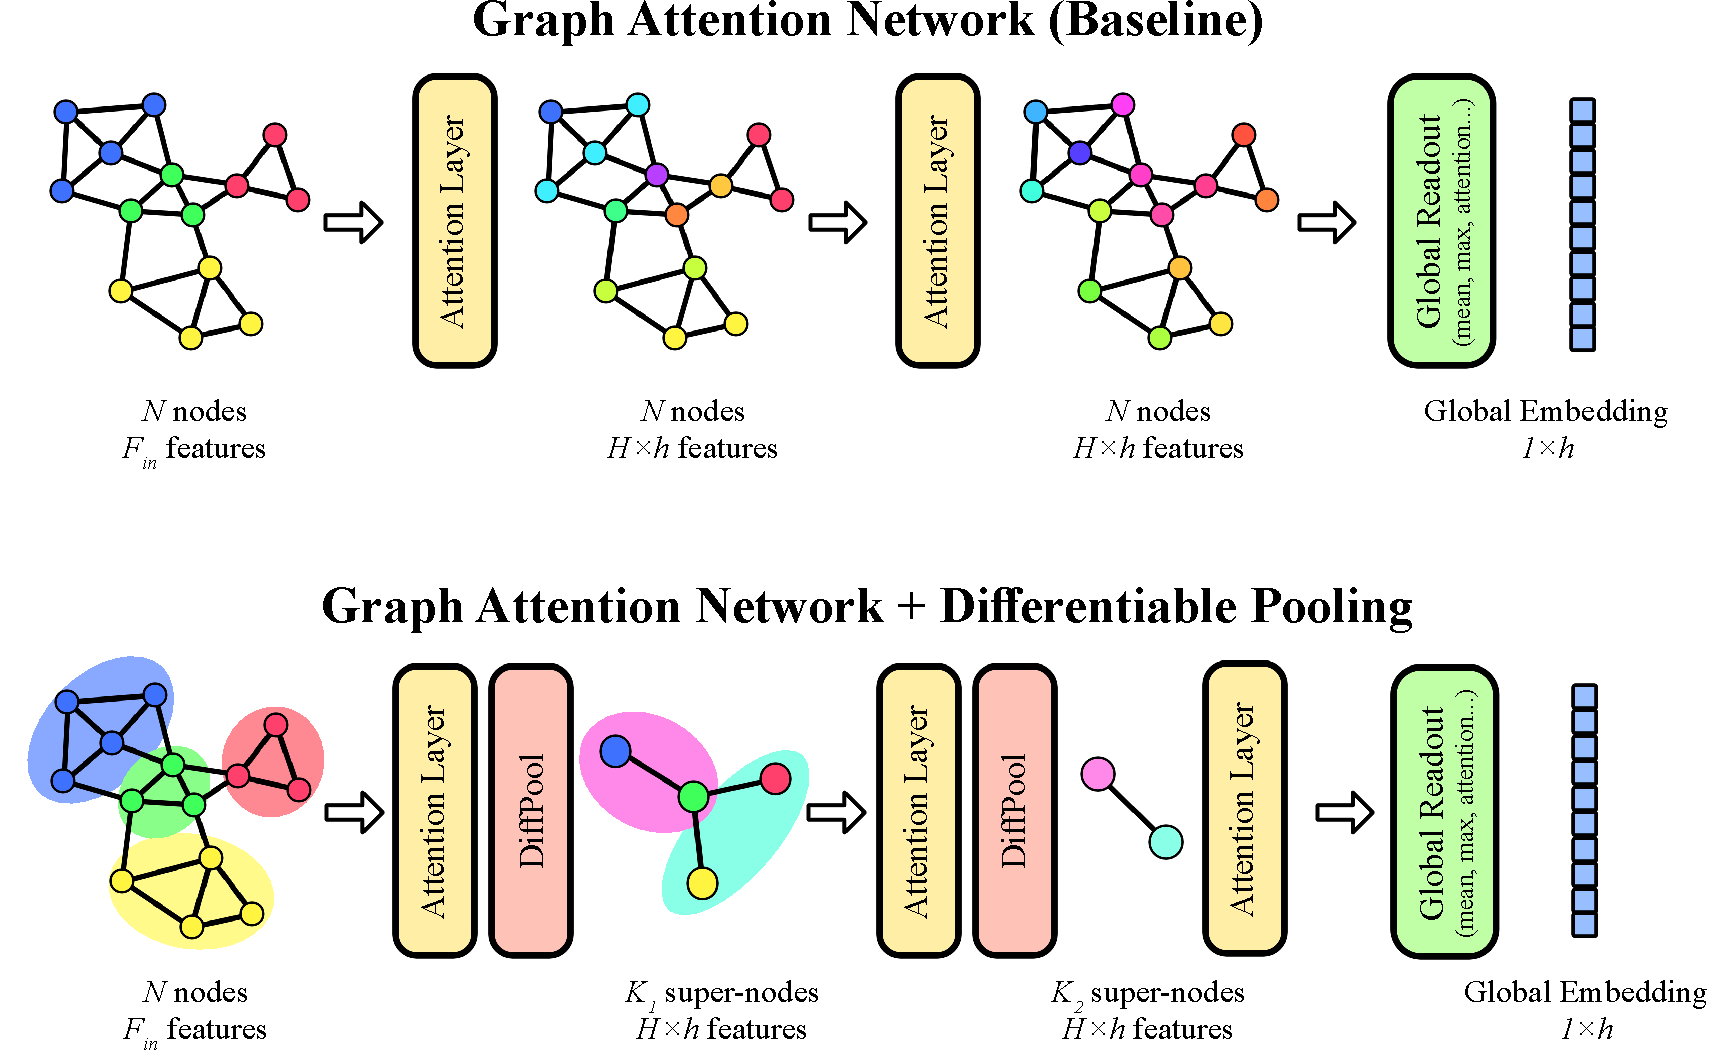
\includegraphics[width=0.8\textwidth]{img/baseline_vs_diffpool.pdf}
    \caption{Comparació visual de les dues arquitectures configurables.
    \textbf{Dalt}: GAT Baseline, on $L \in \{2,3,4\}$ capes d'atenció operen sobre els $N$ nodes
    originals i un \textit{readout} global (mean, max, mean\_max o attention) produeix l'embedding final.
    \textbf{Baix}: GAT+DiffPool, on cada capa GAT va seguida d'un bloc DiffPool ($L_{\text{DP}} \in \{1,2,3\}$
    blocs) que col·lapsa progressivament el graf fins als $K_{L_{\text{DP}}}$ super-nodes finals.}
    \label{fig-diffpool}
\end{figure*}

Com a alternativa, SAGPool~\cite{lee2019selfattentiongraphpooling} selecciona els $K$ nodes més
rellevants via puntuacions d'auto-atenció (selecció discreta, no assignació suau); s'ha preferit
DiffPool per la seva expressivitat contínua i la pèrdua auxiliar de regularització.


\section{Metodologia}

\subsection{Agregació per Pacient (MIL)}
\label{sec:mil}

El diagnòstic és per \textbf{pacient}, no per làmina. Una mateixa secció histològica pot no presentar senyals
visibles de metàstasi si s'analitza aïlladament, mentre que en una altra secció del mateix pacient sí que és
apreciable. Si s'entrena a nivell de làmina, les seccions N1 de pacients N1 que no mostren metàstasi visible
reben un senyal de supervisió incorrecte (N0), contaminant l'entrenament.

Per evitar aquest problema, s'utilitza el paradigma d'\textbf{aprenentatge per múltiples instàncies}
(\textit{Multiple Instance Learning}, MIL): cada pacient es tracta com un \textit{bag} i totes les seves
làmines comparteixen la mateixa etiqueta. El model aprèn a classificar el pacient a partir de les
seves seccions, sense necessitat d'etiquetes individuals per làmina.

Donades les probabilitats $\{p_i = P(\text{N1}_i)\}_{i=1}^{S}$ de les $S$ làmines d'un pacient,
s'implementen quatre estratègies d'agregació:

\begin{itemize}
    \item \textbf{Mean}: $P(\text{N1}_{p}) = \frac{1}{S}\sum_i p_i$. Mitjana aritmètica;
    estratègia escollida per al model final.
    \item \textbf{Noisy-OR}: $P(\text{N1}_{p}) = 1 - \prod_{i=1}^{S}(1 - p_i)$. N'hi ha prou
    amb una làmina amb metàstasi per marcar el pacient com N1.
    \item \textbf{Max}: $P(\text{N1}_{p}) = \max_i\, p_i$. Conservadora, basada en l'evidència
    màxima.
    \item \textbf{Attention MIL}: pes d'atenció aprenent (\textit{gated attention} d'Ilse et
    al.~\cite{ilse2018attentionbaseddeepmultipleinstance}) per a cada làmina a partir del seu
    embedding GAT, i suma ponderada dels embeddings per obtenir la representació del pacient.
\end{itemize}

\subsection{Desbalanceig de Classes i Llindar Operatiu}

El conjunt presenta un fort desbalanceig (N0/N1 $\approx$ 72/28). En detecció de metàstasi, un
fals negatiu és més greu que un fals positiu: l'objectiu clínic és \textbf{maximitzar
l'especificitat mantenint sensibilitat $\approx$ 100\%}, per reduir les cirurgies innecessàries
sense perdre cap N1. S'apliquen tres mecanismes complementaris:
\begin{itemize}\itemsep1pt
  \item \textbf{Partició estratificada} per pacient (manté la proporció N0/N1 a cada subconjunt).
  \item \textbf{Pesos a la \textit{cross-entropy}} amb pes positiu $w_+$ (multiplicador del
        gradient per a la classe N1) com a eix d'optimització, $w_+ \in [1{,}5,\,8]$.
  \item \textbf{Llindar operatiu derivat del val} ($t^*$): es selecciona el llindar més alt
        sobre la corba ROC del \textit{validation set} de cada \textit{fold} que manté
        TPR$=1$; la mediana entre \textit{folds} és el llindar final aplicat al test.
\end{itemize}

\subsection{Esquema d'entrenament i avaluació}
\label{sec:training-scheme}

L'avaluació segueix un esquema en tres etapes que aïlla completament el conjunt de test:

\begin{enumerate}\itemsep1pt
  \item \textbf{Test (15\%):} es separa des de la construcció dels grafs i \textbf{mai
        s'usa} per a selecció d'hiperparàmetres ni \textit{early stopping}.
  \item \textbf{Cerca bayesiana + CV 5-\textit{fold}} sobre el 85\% restant: cada configuració
        s'avalua amb \textit{Stratified K-Fold} per pacient i \textit{early stopping}
        (\textit{patience}$=\!20$). L'objectiu maximitzat és
        $\overline{\text{spec}}_{\text{CV}} - 10\cdot\max(0, 1-\overline{\text{sens}}_{\text{CV}})$:
        especificitat mitjana penalitzant fortament caigudes de sensibilitat (vegeu Annex
        \ref{app:sweep-config}).
  \item \textbf{Entrenament final i avaluació al test:} amb els millors hiperparàmetres,
        el 85\% es torna a dividir 90/10 per fer \textit{early stopping} intern, i el model
        final s'avalua una sola vegada al test (15\%) amb el llindar $t^*$ mediana de les 5
        $t^*$ obtingudes als folds CV.
\end{enumerate}

\textbf{Cerca bayesiana.} S'utilitza el \textit{Tree-structured Parzen Estimator}~(TPE) sobre
$\sim$15 eixos. Els \textbf{200 primers trials} ($\sim$10$\times$ dimensions) són mostreig uniforme
aleatori (exploració); després el TPE explota l'historial. Tots els mostratges, \textit{folds} CV i
inicialització de pesos usen \textit{seed} fixa. L'estudi és persistent (\texttt{SQLite}) i reprenible;
l'espai complet es recull a l'Annex \ref{app:sweep-config}. \textbf{El conjunt de test (15\%) no es
toca en cap pas del sweep}; només es carrega al pas de finalització, una sola vegada.

\section{Resultats}

Les mètriques principals són l'\textbf{AUC-ROC} (ordenació global independent del llindar)
i les \textbf{mètriques clíniques}: \textbf{sensibilitat} ($\text{VP}/(\text{VP}+\text{FN})$)
i \textbf{especificitat} ($\text{VN}/(\text{VN}+\text{FP})$). En detecció de metàstasi, la
sensibilitat és la més rellevant: un fals negatiu (no tractar un N1) és més greu que un
fals positiu.

\textbf{Pregunta central.} Aquest TFG vol respondre, sobre les dades disponibles, si el
\textbf{GAT Baseline} (\textit{readout} global pla després de les capes GAT) o el
\textbf{GAT+DiffPool} (reducció jeràrquica del graf abans del \textit{readout}) és
preferible per al diagnòstic N0/N1, i quina configuració d'hiperparàmetres maximitza
el rendiment al test. Per arribar-hi s'han combinat dues estratègies: (i) dos estudis
Optuna TPE aïllats per arquitectura (Annex~\ref{app:sweep-config}, eixos compartits i
específics per branca) i (ii) una exploració per graella exhaustiva més acotada sobre
GAT Baseline (255 configuracions, només eixos arquitectònics i de regularització).

\textbf{Volum d'experiments.} El sweep TPE va avaluar $N_{\text{base}}=350$ \textit{trials}
GAT Baseline i $N_{\text{diff}}=231$ GAT+DiffPool (581 totals; 499 complets, 82 \textit{pruned},
1 fallit). El grid va avaluar 255 configuracions de GAT Baseline. Per a la comparació
final, s'han re-avaluat les millors configuracions de cada estratègia amb el
\textbf{procediment estricte sense data leakage} (5-fold StratifiedKFold sobre el pool +
retrain final 90/10 + avaluació única al test). La Taula~\ref{tab:configs-compare}
resumeix les configuracions més rellevants.

\begin{table*}[t]
\centering
\caption{Comparació de configuracions re-avaluades amb procediment estricte sense data
leakage (5-fold CV + retrain final 90/10 + test). \textbf{Files ressaltades}: model
seleccionat (\textit{grid1}) per màxima AUC CV i mantenir sens.\ $=100\%$ al test amb
millor especificitat. Grid \#1/\#5 corresponen a configs del grid antic (255
configs), \textit{sweep} a les millors del TPE bayesià.}
\label{tab:configs-compare}
\small
\begin{tabular}{lccccccc}
\toprule
\textbf{Config} & \textbf{Arq.} & \textbf{Pooling/MIL}
  & \textbf{$h$/$H$/drop} & \textbf{AUC CV} & \textbf{AUC test}
  & \textbf{Sens/Espec @$t^*$} & \textbf{Sens/Espec @0,5} \\
\midrule
\textbf{Grid \#1 (sel.)} & \textbf{Base.} & \textbf{att/mean}      & $\mathbf{256/4/0{,}3}$ & $\mathbf{0{,}862\!\pm\!0{,}038}$ & $\mathbf{0{,}875}$ & $\mathbf{1{,}00\,/\,0{,}575}$ & $\mathbf{0{,}562\,/\,0{,}925}$ \\
Grid \#5                & Baseline & att/mean      & $256/2/0{,}1$ & $0{,}836\!\pm\!0{,}050$ & $0{,}892$ & $1{,}00\,/\,0{,}375$ & $0{,}688\,/\,0{,}900$ \\
Sweep Baseline \#303    & Baseline & mm/att        & $128/4/0{,}36$ & $0{,}843\!\pm\!0{,}026$ & $0{,}816$ & $0{,}69\,/\,0{,}825$ & $0{,}438\,/\,0{,}900$ \\
Sweep DiffPool \#199    & DiffPool & diff/mean     & $128/2/0{,}44$ & $0{,}847\!\pm\!0{,}048$ & $0{,}786$ & $0{,}63\,/\,0{,}700$ & $0{,}500\,/\,0{,}825$ \\
DiffPool aux=$0{,}01$   & DiffPool & diff/mean     & $128/2/0{,}40$ & $0{,}844\!\pm\!0{,}035$ & $0{,}805$ & $0{,}81\,/\,0{,}725$ & $0{,}562\,/\,0{,}900$ \\
\bottomrule
\end{tabular}\\[2pt]
\footnotesize{Pooling: att = attention, mm = mean\_max, diff = DiffPool jeràrquic.
MIL: mean = mitjana, att = attention MIL.
Llindar $t^*$ derivat com a mediana dels 5 llindars del val set
(sens=$100\%$ a cada fold), aplicat al test sense reajustar.}
\end{table*}

\textbf{Lectura dels resultats.} El sweep TPE \textbf{no supera el grid recuperat}
tot i avaluar $2{,}3\!\times$ més configuracions (581 vs 255 trials): el millor del
sweep (DiffPool \#199, AUC test $0{,}786$) queda 9 punts per sota del Grid \#1
($0{,}875$). Amb dataset petit ($n_{\text{pool}}\!=\!311$), la cerca bayesiana és més
vulnerable a sobreajustar el val set; el TPE pot triar configuracions "afortunades" al
CV que no es transfereixen al test. Dues configuracions del grid (\#1 i \#5)
\textbf{mantenen sens.\ $=100\%$ al test} amb el llindar $t^*$, cosa que cap del sweep
aconsegueix. Finalment, el \textbf{GAT Baseline supera GAT+DiffPool} en aquest dataset:
les seccions tenen pocs centenars de \textit{patches} i la reducció jeràrquica a
super-nodes elimina més informació que la que sintetitza (la variant
$\lambda_{\text{aux}}\!=\!0{,}01$ tot just arriba a AUC test $0{,}805$).

\textbf{Model seleccionat.} Es tria \textbf{Grid \#1} per al \textit{reporting} final:
GAT Baseline amb pooling \textit{attention}, MIL \textit{mean}, $h=256$, $H=4$,
\textit{dropout} $0{,}3$, $\lambda_{\text{wd}}=10^{-4}$, $\eta=3\!\cdot\!10^{-4}$ i
optimitzador Adam amb \textit{ReduceLROnPlateau}. AUC CV $0{,}862\pm 0{,}038$, AUC
test $0{,}875$, sensibilitat $100\%$ al test (els $16$ casos N1 detectats), especificitat
$57{,}5\%$.

\begin{table}[h]
\centering
\caption{Matriu de confusió del \textbf{model seleccionat} (Grid \#1) al conjunt de
test ($n=56$) amb el llindar $t^*=0{,}133$.
Mètriques clíniques: sensibilitat $=1{,}000$ (16/16 N1 detectats),
especificitat $=0{,}575$, VPP $=0{,}485$, VPN $=1{,}000$.}
\label{tab:cm}
\small
\begin{tabular}{llcc}
\toprule
 & & \multicolumn{2}{c}{\textbf{Diagnòstic real}} \\
 & & \textbf{N0} & \textbf{N1} \\
\midrule
\multirow{2}{*}{\textbf{Predicció}}
  & \textbf{N0} & 23 & 0 \\
  & \textbf{N1} & 17 & 16 \\
\bottomrule
\end{tabular}
\end{table}

\subsection{Importància dels hiperparàmetres per arquitectura}
\label{sec:main-effects}

Cada estudi Optuna calcula automàticament la \textbf{importància de cada eix d'optimització}
amb \textit{fANOVA}, una descomposició funcional de la variància de l'objectiu CV explicada
per cada hiperparàmetre. L'Annex~\ref{app:main-effects} presenta la taula completa
(columnes \textbf{Baseline} i \textbf{DiffPool} costat a costat). Aquí destaquem els eixos
amb importància $> 10\,\%$ en almenys una arquitectura.

\textbf{GAT Baseline.} L'agregació MIL domina l'objectiu de manera molt clara
($I=0{,}64$): cap altre eix supera el $10\%$. Curiosament, el sweep TPE prefereix
\textit{attention} MIL ($90\%$ del top 10\%), mentre que \textbf{el model que millor
generalitza al test} (Grid \#1) usa \textit{mean} MIL: una mostra més que l'objectiu CV
no prediu bé el test amb aquesta mida de dades.

\textbf{GAT+DiffPool.} La importància es distribueix molt més: MIL és encara el primer
($0{,}22$), seguit del pes del penalty auxiliar $\lambda_{\text{aux}}$ ($0{,}14$),
$\eta$ ($0{,}13$), $\lambda_{\text{wd}}$ ($0{,}08$) i \textit{dropout} ($0{,}08$). El
sweep convergeix a $\lambda_{\text{aux}}\!\approx\!0{,}1$ (límit inferior del rang),
suggerint que un rang més ampli ($[10^{-3}, 10]$) podria explorar zones encara millors.
Una variant amb $\lambda_{\text{aux}}=0{,}01$ (fora del rang del sweep) ja millora
lleugerament l'AUC test del millor DiffPool del sweep (de $0{,}786$ a $0{,}805$;
vegeu Taula~\ref{tab:configs-compare}).

\subsection{Comparació amb guies clíniques i SOTA}
\label{sec:resultats-comparacio}

La Taula~\ref{tab:comparison} situa el \textbf{model seleccionat} (Grid \#1, vegeu
Taula~\ref{tab:configs-compare}) davant de les guies clíniques de referència (Secció~\ref{sec:guidelines-sota}) i del model de IA de referència.
Les xifres de les guies provenen de~\cite{tanino2024comparative} ($n\!=\!560$),
i les del GAT s'han obtingut sobre el test d'aquest treball ($n\!=\!56$;
prevalença N1 $28{,}6\%$, superior a la clínica real $\sim\!8$–$15\%$
\cite{zaffalon2023}). Sensibilitat i especificitat són independents de la
prevalença i són la base de la comparació; el VPP s'ha d'interpretar amb
cautela (Secció~\ref{sec:limitacions}).

\begin{table*}[h]
\centering
\caption{Comparació de rendiment entre el model proposat, les guies clíniques i l'estat
de l'art. \textbf{Guies:} Tanino et al.~\cite{tanino2024comparative} ($n\!=\!560$, Hiroshima).
\textbf{IBC Score:} Dawson et al.~\cite{dawson2024budding} ($n\!=\!565$, multicèntric).
\textbf{LightGBM:} Piao et al.~\cite{piao2023ai} ($n\!=\!105$ test, variables clinicopat.).
\textbf{GAT:} aquest treball ($n\!=\!56$ test).
Estudis i poblacions independents; el PPV no és directament comparable
(prevalença N1 diferent entre estudis).
Bal.Acc. $= (S\!+\!E)/2$; calculada per a les guies i l'IBC Score a partir de Sens./Espec.
reportades.} % [NEW: comparison]
\label{tab:comparison}
\small
\begin{tabular}{llrrrr}
\toprule
\textbf{Sistema} & \textbf{Tipus d'entrada} & \textbf{Sens.} & \textbf{Espec.} & \textbf{AUC} & \textbf{Bal.Acc.} \\
\midrule
\multicolumn{6}{l}{\textit{Guies i puntuació clínica}} \\[2pt]
JSCCR \cite{jsccr2019}        & Guia clínica  & $100\%$ & $19\%$  & $0{,}596$ & $59{,}5\%$ \\
NCCN                           & Guia clínica  & $98\%$  & $52\%$  & $0{,}749$ & $75{,}0\%$ \\
ESMO \cite{esge2022}           & Guia clínica  & $98\%$  & $50\%$  & $0{,}743$ & $74{,}0\%$ \\
IBC Score \cite{dawson2024budding} & Puntuació histopat. & $90\%$ & $26\%$ & $0{,}68$ & $58{,}0\%$ \\
\midrule
\multicolumn{6}{l}{\textit{Models d'IA}} \\[2pt]
LightGBM \cite{piao2023ai}                          & Var.\ clinicopatol. & $100\%$  & $85{,}8\%$ & $0{,}960$ & $92{,}9\%$ \\
\textbf{GAT (aquest TFG, llindar $0{,}5$)}          & \textbf{Imatge WSI} & $56{,}2\%$ & $92{,}5\%$ & $0{,}875$ & $74{,}4\%$ \\
\textbf{GAT (aquest TFG, llindar $t^*\!=\!0{,}133$)$^{\dagger}$} & \textbf{Imatge WSI} & $\mathbf{100\%}$ & $57{,}5\%$ & $0{,}875$ & $78{,}8\%$ \\
\bottomrule
\end{tabular}\\[2pt]
\footnotesize{$^{\dagger}$\,$t^*$ s'ha determinat com a mediana dels 5 llindars dels \textit{val sets}
dels folds CV (sens=$100\%$ en cada fold), aplicat al test sense reajustar (procediment
sense \textit{data leakage}). Model: Grid \#1 (vegeu Taula~\ref{tab:configs-compare}).}
\end{table*}

En la detecció de metàstasi, un fals negatiu (no tractar un pacient N1) és un error inacceptable,
mentre que un fals positiu (cirurgia innecessària) és recuperable. Per això el punt operatiu
desitjat és el que toca \textbf{la part superior} (sens.\ $=\!100\%$) i alhora queda \textbf{tan
a l'esquerra com sigui possible} (espec.\ màxima). La Figura~\ref{fig:roc-top5} superposa les
corbes ROC dels models més rellevants amb els punts operatius de les guies clíniques.

\begin{figure}[h]
\centering
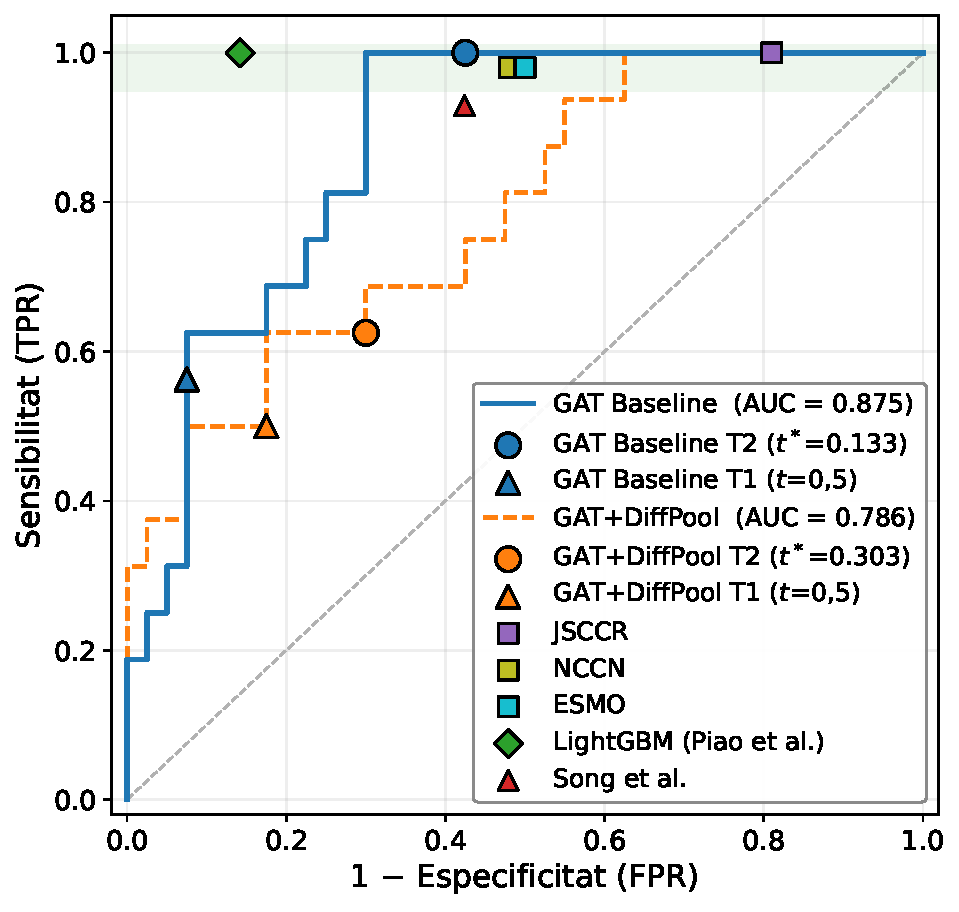
\includegraphics[width=0.48\textwidth]{img/roc_top5.pdf}
\caption{Corbes ROC al conjunt de test (56 pacients) dels models comparats: \textbf{Grid \#1}
(GAT Baseline; model seleccionat; AUC $=0{,}875$), Grid \#5 (AUC $=0{,}892$), sweep Baseline
\#303 (AUC $=0{,}816$) i sweep DiffPool \#199 (AUC $=0{,}786$). El cercle gros marca el
llindar $t^*\!=\!0{,}133$ del model seleccionat (Grid \#1), que assoleix sens.\ $=100\%$ i
espec.\ $=57{,}5\%$ al test. $t^*$ s'ha derivat exclusivament del val set sense \textit{data
leakage}. Es marquen els punts operatius publicats de JSCCR, NCCN, ESMO (quadrats) i
LightGBM (diamant).}
\label{fig:roc-top5}
\end{figure}

\textbf{Impacte clínic.} El llindar $t^*$ manté \textbf{sens.\ $=100\%$ al test} (16/16 N1
detectats, $\text{VPN}\!=\!1{,}000$), amb espec.\ $57{,}5\%$. La literatura estima que el
$80$–$90\%$ de les cirurgies actuals en pT1 són innecessàries~\cite{MartinezDeJuan2024},
coherent amb les especificitats del $19$–$52\%$ de les guies. Mantenint sens.\ $=100\%$, el
GAT redueix les cirurgies innecessàries de $\sim\!81$ (JSCCR) o $\sim\!49$ (NCCN/ESMO) a
$\sim\!42{,}5$ per cada $100$ pacients N0. Sobre els $40$ N0 del test, són $17$ FP en lloc
dels $\sim\!32$ de JSCCR. Al llindar $0{,}5$ la sensibilitat és inferior ($56{,}2\%$); $t^*$
és el que fa el model clínicament útil.

\section{Implementació i Eines}

La implementació segueix un disseny modular: la construcció de grafs, el model, el codi
d'entrenament i el \textit{sweep} bayesià estan desacoblats. La configuració es gestiona via YAML i,
per a la cerca, via \texttt{Optuna} amb \textit{storage} \texttt{SQLite} reprenible. Codi accessible
a~\cite{morillo2026codi}.

\textbf{Frontend web.} S'ha desenvolupat una interfície (FastAPI + JS sense \textit{build step}) que
ofereix: (a) \textbf{visualització del WSI} amb superposició dels \textit{patches} i la màscara
anotada; (b) \textbf{visualització dels grafs} de Delaunay sobre la imatge, amb pesos d'atenció per
node (mitjana sobre els $H$ caps de l'última capa GAT, $\in [0,1]$ ja que GAT fa \textit{softmax}
sobre veïns); (c) \textbf{selector de model} que carrega qualsevol \textit{checkpoint} dels
\textit{trials} del sweep i n'infereix automàticament l'arquitectura des dels pesos; (d) \textbf{mode
d'inferència} amb desglossament de la propagació capa a capa (mode depuració); i (e) \textbf{pestanya
d'estadístiques} amb corbes ROC/PR, matriu de confusió i mètriques per classe al test, generades
sense \textit{data leakage}. El diagrama de blocs detallat del pipeline és la
Figura~\ref{fig:pipeline-full} de l'Annex~\ref{app:pipeline-full}.

\section{Conclusions}

\subsection{Conclusions}

En aquest TFG s'ha construït un sistema complet de classificació N0/N1 per a càncer
colorrectal pT1 a partir de WSI, que inclou la generació de grafs espacials de Delaunay,
l'entrenament del model GAT amb dues estratègies de cerca d'hiperparàmetres (graella
exhaustiva acotada $+$ sweep bayesià TPE), i l'avaluació final sobre un conjunt de test
fix (56 pacients). La pregunta central \textbf{«GAT Baseline o GAT+DiffPool, i amb
quina configuració?»} es respon a partir de la Taula~\ref{tab:configs-compare}:
\textbf{el GAT Baseline amb la configuració Grid \#1} (\textit{attention pooling},
MIL \textit{mean}, $h\!=\!256$, $H\!=\!4$, dropout $0{,}3$, $\lambda_{\text{wd}}=10^{-4}$)
obté el millor balanç: AUC test $=0{,}875$, sensibilitat $100\%$ (els 16 N1 detectats) i
especificitat $57{,}5\%$ al llindar $t^*\!=\!0{,}133$ derivat del val set. Se'n destaquen
tres observacions:

\begin{itemize}
  \item \textbf{El sweep TPE no supera el grid recuperat}. Tot i avaluar 2,3$\times$ més
  configuracions (581 vs 255 trials) i cobrir més eixos, el millor model del sweep (DiffPool
  \#199) queda 9 punts d'AUC test per sota del Grid \#1 ($0{,}786$ vs $0{,}875$). Amb un
  dataset petit ($n_{\text{pool}}=311$), la cerca bayesiana és més vulnerable a sobreajustar
  el val set, especialment quan l'objectiu ($\overline{\text{spec}} - 10\cdot\max(0,
  1\!-\!\overline{\text{sens}})$) prioritza un punt operatiu concret que pot no transferir-se
  al test.
  \item \textbf{El GAT Baseline supera el GAT+DiffPool} amb aquest dataset. Les seccions
  contenen pocs centenars de \textit{patches}; la reducció jeràrquica a super-nodes
  ($K_{\text{top}}\!=\!50$, $K_{\text{bot}}\!=\!3$) elimina més informació que la que
  sintetitza. Una variant amb $\lambda_{\text{aux}}\!=\!0{,}01$ (fora del rang del sweep)
  millora lleugerament el DiffPool ($0{,}805$ AUC) però no arriba al nivell del Baseline.
  \item \textbf{Robustesa del llindar}. El Grid \#1 i altres dues configuracions del grid
  (\#5 i \#5+AdamW) mantenen sens.\ $=100\%$ al test amb el llindar $t^*$ del val set,
  cosa que cap configuració del sweep aconsegueix. Aquesta propietat és la que fa el
  sistema clínicament útil com a filtre de descartament: amb $\text{VPN}\!=\!1{,}000$ al
  test, un resultat negatiu del model permet evitar la cirurgia amb seguretat sobre la
  mostra avaluada.
\end{itemize}

\subsection{Discussió Comparativa}

L'AUC de test del model seleccionat ($0{,}875$) supera la de JSCCR ($0{,}596$), NCCN
($0{,}749$) i ESMO ($0{,}743$)~\cite{tanino2024comparative}. L'especificitat al llindar
$t^*$ ($57{,}5\%$) és superior a la de JSCCR ($19\%$) i comparable a NCCN/ESMO ($50$–$52\%$)
mantenint la sensibilitat al $100\%$.

\textbf{VPP i ajust per prevalença.}
El VPP de $48{,}5\%$ s'ha calculat amb la prevalença del test ($28{,}6\%$ N1),
superior a la clínica real ($\sim\!8$–$15\%$) \cite{zaffalon2023}. A una prevalença del
$10\%$, el VPP baixa a $\sim\!21\%$ i el VPN es manté al $100\%$ (càlcul per Bayes amb
Sens./Espec.\ observades: $1{,}000/0{,}575$). El model és, doncs, especialment útil com a
\textbf{filtre de descartament}: un resultat negatiu té probabilitat 1 de ser correcte
sobre aquesta mostra, i podria evitar la cirurgia amb seguretat. Sensibilitat i
especificitat, independents de la prevalença, segueixen sent les mètriques comparatives
més robustes.

\textbf{Sensibilitat ajustable per llindar.}
Al llindar per defecte ($0{,}5$) la sensibilitat al test és inferior ($56{,}2\%$) però
l'especificitat puja al $92{,}5\%$. Ajustant el llindar a $t^*\!=\!0{,}133$ (derivat
exclusivament del val set, vegeu Limitació~4), el GAT assoleix sensibilitat $100\%$ i
especificitat $57{,}5\%$, una millora de $38{,}5$ punts sobre JSCCR al mateix nivell de
sensibilitat.

\textbf{Comparació amb IA SOTA.}
El model de gradient boosting (\textit{LightGBM}) de Piao et al.~\cite{piao2023ai},
entrenat amb $\sim\!10\!\times$ més dades i amb accés a variables clinicopatològiques
estructurades, obté Sens.$=\!100\%$ amb Espec.$=\!85{,}8\%$ i AUC $0{,}960$. El GAT, al
mateix punt operatiu de sensibilitat, arriba a Espec.\ $57{,}5\%$ ($28$ punts per sota),
però amb la imatge WSI com a única entrada. Els dos models són complementaris: el GAT
pot córrer just després d'escanejar la làmina, sense esperar el report patològic; el
model basat en \textit{LightGBM} requereix les variables clinicopatològiques ja anotades.

\textbf{Cerca bayesiana vs graella en datasets petits.}
Una observació metodològica rellevant: en aquest treball, el sweep TPE bayesià (581 trials,
17 eixos) \textbf{no ha trobat un model millor} que la graella exhaustiva acotada (255
configs, 6 eixos). Una hipòtesi: amb dataset petit ($n_{\text{pool}}\!=\!311$), la
variància entre splits CV ($\sigma_{\text{spec}}\!\approx\!0{,}10$–$0{,}20$) domina
sobre el guany d'una exploració més fina, i el TPE pot triar configuracions
"afortunades" al val set que no es transfereixen. La graella, en canvi, va explorar un
nombre menor de configuracions "robustes" que generalitzen millor.

\subsection{Limitacions}
\label{sec:limitacions}

\textbf{(1) Mida del test.}
Amb $56$ pacients al test (només $16$ N1), els intervals de confiança al $95\%$ de l'AUC
són amplis ($\pm\!0{,}07$–$0{,}10$). L'AUC CV del model seleccionat ($0{,}862\!\pm\!0{,}038$)
i l'AUC test ($0{,}875$) són consistents, però la variància de l'especificitat al CV és alta
(mitjana $0{,}369\!\pm\!0{,}198$ amb el llindar $t^*$), reflectint la inestabilitat
entre folds. Caldria un test més gran per a conclusions clíniques robustes.

\textbf{(2) Absència de validació externa.}
El dataset prové de $26$ hospitals espanyols, però no s'ha provat sobre dades d'un centre
independent. Campanella et al.~\cite{campanella2019} reporten, en models MIL de patologia,
caigudes de $3$–$6$ punts d'AUC en escàners externs i fins a $7$ punts en canvis de
domini institucional. L'aplicabilitat clínica requereix, per tant, validació externa.

\textbf{(3) Desbalanceig de prevalença.}
La prevalença N1 al test ($28{,}6\%$) supera la clínica real ($\sim\!8$–$15\%$); el VPP
s'ha d'interpretar amb cautela (Discussió Comparativa).

\textbf{(4) Selecció del llindar i biaix del val set.}
Per maximitzar la sensibilitat, s'ha buscat el primer punt de la corba ROC del val set de
cada fold del model seleccionat (Grid \#1) en què TPR$=\!1{,}0$, i s'ha pres la mediana
sobre els 5 folds com a $t^*\!=\!0{,}133$. Aplicat al test, manté sens.\ $=\!100\%$
amb espec.\ $=57{,}5\%$. El val set ja s'havia usat per a \textit{early stopping}, per
la qual cosa $t^*$ pot tenir un biaix lleugerament optimista; idealment, hauria de
fixar-se sobre un val set extern. La variància del llindar entre folds també és alta
($\sigma_{t^*}\!\approx\!0{,}08$), reflectint la sensibilitat del procediment a la
divisió de dades.


\printbibliography

\clearpage
\onecolumn
\appendix

\section*{Apèndix}

\setcounter{section}{1}

\subsection{Diagrama de flux detallat del \textit{pipeline}}
\label{app:pipeline-full}

\begin{figure}[H]
\centering
\begin{tikzpicture}[
    node distance=0.45cm,
    box/.style={rectangle, rounded corners=3pt, draw,
                minimum width=2.2cm, minimum height=0.65cm,
                align=center, font=\small},
    ext/.style={box, draw=gray!55, fill=gray!12},
    own/.style={box, draw=blue!65!black, line width=1.3pt, fill=blue!7},
    arr/.style={->, >=stealth, thick},
    lbl/.style={font=\small\bfseries\sffamily, align=center},
]

%% Columna 1: Preparació de dades
\node[ext] (wsi)  {WSI};
\node[ext, below=of wsi] (sw)   {\textit{Sliding}\\window};
\node[ext, below=of sw]  (pat)  {Patches $2048{\times}2048$};
\node[ext, below=of pat] (uni)  {\textit{UNI2}};
\node[ext, below=of uni] (cls)  {\textit{CLS} 1536-dim};

\foreach \a/\b in {wsi/sw, sw/pat, pat/uni, uni/cls}
  \draw[arr] (\a)--(\b);

%% Columna 2: Construcció del graf
\node[own, right=2.4cm of wsi] (coo) {Coord. $(i,j)$};
\node[own, below=of coo]       (del) {Delaunay};
\node[own, below=of del]       (pru) {Poda $>2{\times}\bar{d}$};
\node[own, below=of pru]       (gra) {\textbf{Graf} $(\mathbf{X},\mathbf{A})$};

\foreach \a/\b in {coo/del, del/pru, pru/gra}
  \draw[arr] (\a)--(\b);
\draw[arr] (pat.east) to[out=0, in=180] (coo.west);
\draw[arr] (cls.east) to[out=0, in=180] (gra.west);

%% Columna 3: Model
\node[own, right=2.4cm of coo] (mod)  {GATClassifier};
\node[own, below=of mod]       (pn1)  {$P(\text{N1})$ per graf};
\node[own, below=of pn1]       (agg)  {Agregació MIL};
\node[own, below=of agg]       (diag) {$P(\text{N1})$ per pacient};

\foreach \a/\b in {mod/pn1, agg/diag}
  \draw[arr] (\a)--(\b);
\draw[arr] (pn1) -- node[right, font=\scriptsize]{${\times}S$} (agg);
\draw[arr] (gra.east) to[out=0, in=180] (mod.west);

%% Hiperparàmetres associats (caixes vermelles dashed) a la dreta dels blocs configurables
\node[draw, dashed, rounded corners=2pt, fill=red!4, font=\sffamily\scriptsize, align=left,
      right=0.7cm of mod, minimum width=3.2cm]
      (h-mod) {$L,\ h,\ H,\ p_{\text{drop}}$,\\\textit{pooling},
               $L_{\text{DP}},K_\ell,\lambda_{\text{aux}}$};
\node[draw, dashed, rounded corners=2pt, fill=red!4, font=\sffamily\scriptsize, align=left,
      right=0.7cm of agg, minimum width=3.2cm]
      (h-agg) {MIL: mean/max/\\noisy-OR/attention};
\node[draw, dashed, rounded corners=2pt, fill=red!4, font=\sffamily\scriptsize, align=left,
      right=0.7cm of diag, minimum width=3.2cm]
      (h-diag) {Llindar $t^*$\\$\in [0,1]$ (val.)};
\node[draw, dashed, rounded corners=2pt, fill=red!4, font=\sffamily\scriptsize, align=left,
      right=0.7cm of pru, minimum width=3.2cm]
      (h-pru) {\textit{factor poda}};
\foreach \a/\b in {mod/h-mod, agg/h-agg, diag/h-diag, pru/h-pru}
  \draw[densely dotted] (\a) -- (\b);

%% Ground truth
\node[ext, below=0.9cm of diag] (exc) {Excel diagnòstic real};
\draw[arr] (exc.north) -- (diag.south);

%% Etiquetes de columna
\node[lbl, above=0.55cm of wsi] {\footnotesize Preparació\\de dades};
\node[lbl, above=0.55cm of coo] {\footnotesize Construcció\\del graf};
\node[lbl, above=0.55cm of mod] {\footnotesize Model};
\node[lbl, above=0.55cm of h-mod] {\footnotesize Hiperparàm.};
\node[lbl, left=0.35cm of exc.west, anchor=east] {\footnotesize Ground\\truth};

\end{tikzpicture}
\caption{Diagrama de flux del \textit{pipeline} complet amb hiperparàmetres optimitzats per
la cerca bayesiana (columna dreta, caixes vermelles discontínues). \textit{Blocs grisos}: etapes
realitzades pels companys de l'equip i dades de referència. \textit{Blocs blaus}:
contribucions d'aquest TFG. La fletxa ${\times}S$ indica que les $S$ seccions d'un
pacient es processen com a grafs independents i les $P(\text{N1})$ s'agreguen via MIL
per obtenir el diagnòstic per pacient, que es compara amb el diagnòstic real de l'Excel.
$L$: capes GAT; $h$: dim. oculta; $H$: caps d'atenció; $L_{\text{DP}}$: blocs DiffPool;
$K_\ell$: super-nodes per nivell; $\lambda_{\text{aux}}$: pes del penalty DiffPool; $t^*$:
llindar de decisió derivat del val set.}
\label{fig:pipeline-full}
\end{figure}

\newpage

\subsection{Variants d'arquitectura del \textit{GATClassifier}}
\label{app:model-variants}

El diagrama~\ref{fig:gat-variants} mostra com un \textbf{mateix graf d'entrada}
pot ser processat de maneres molt diverses depenent de la configuració: les
caixes blaves representen capes apreses i les taronges discontínues els eixos
d'optimització configurables.

\begin{figure}[H]
\centering
\begin{tikzpicture}[
    bblue/.style={rectangle, rounded corners=3pt,
                  draw=blue!65!black, line width=1.2pt, fill=blue!7,
                  minimum width=3.9cm, minimum height=0.6cm,
                  align=center, font=\small},
    opt/.style={rectangle, rounded corners=2pt,
                draw=orange!70!black, dashed, fill=orange!5,
                minimum width=3.9cm,
                align=center, font=\sffamily\scriptsize},
    inp/.style={rectangle, rounded corners=3pt,
                draw=green!60!black, fill=green!8,
                minimum width=8.2cm, minimum height=0.6cm,
                align=center, font=\small},
    mid/.style={rectangle, rounded corners=3pt,
                draw=orange!60!black, fill=yellow!10,
                minimum width=8.2cm, minimum height=0.6cm,
                align=center, font=\small},
    out/.style={rectangle, rounded corners=3pt,
                draw=red!60!black, fill=red!8,
                minimum width=8.2cm, minimum height=0.6cm,
                align=center, font=\small},
    arr/.style={->, >=stealth, thick},
]

%% ─── Input ──────────────────────────────────────────────────────────────────
\node[inp] (in) at (0,0)
    {\textbf{Graf} $\mathcal{G}=(\mathbf{X},\mathbf{A})$
     \;—\; $N$ nodes $\times$ 1\,536 feat.};

%% ─── BASELINE (left) ────────────────────────────────────────────────────────
\node[font=\small\bfseries\sffamily, text=blue!70!black]
     at (-4.4,-1.3) {\footnotesize\textsc{Baseline}};

\node[bblue] (b_gat) at (-4.4,-2.0)
    {GAT$_1 \to \cdots \to$ GAT$_L$};

\node[opt, below=0.35cm of b_gat] (b_gat_opt)
    {$L\!\in\!\{2,3,4\}$;\quad$h\!\in\!\{64,128,256\}$\\
     $H\!\in\!\{2,4\}$;\quad drop.$\,\in[0{,}05,\,0{,}5]$};

\node[bblue, below=0.35cm of b_gat_opt] (b_ro)
    {\textit{Readout} global};

\node[opt, below=0.35cm of b_ro] (b_ro_opt)
    {mean $\cdot$ max $\cdot$ sum\\
     mean\_max $\cdot$ attention};

%% ─── DIFFPOOL (right) ───────────────────────────────────────────────────────
\node[font=\small\bfseries\sffamily, text=blue!70!black]
     at (4.4,-1.3) {\footnotesize\textsc{DiffPool}};

\node[bblue] (d_gat1) at (4.4,-2.0)
    {GAT$_1$};

\node[bblue, below=0.35cm of d_gat1] (d_dp1)
    {DiffPool$_1$:\;\;$N\!\to\!K_1$};

\node[font=\scriptsize, below=0.15cm of d_dp1] (d_vdots)
    {$\vdots$\quad($L_{\text{DP}}$ blocs)};

\node[bblue, below=0.15cm of d_vdots] (d_dpn)
    {DiffPool$_{L_{\text{DP}}}$:\;\;$\cdots\!\to\!K_{L_{\text{DP}}}$};

\node[bblue, below=0.35cm of d_dpn] (d_gatn)
    {GAT$_{L_{\text{DP}}+1}$};

\node[opt, below=0.35cm of d_gatn] (d_dp_opt)
    {$L_{\text{DP}}\!\in\!\{1,2,3\}$;\;
     $K_{\text{top}}\!\in\!\{10,25,50\}$\\
     $K_{\text{bot}}\!\in\!\{3,5,10\}$;\;
     $\lambda_{\text{aux}}\!\in\![0{,}1,10]$};

\node[bblue, below=0.35cm of d_dp_opt] (d_ro)
    {\textit{Diff readout} final};

\node[opt, below=0.35cm of d_ro] (d_ro_opt)
    {mean $\cdot$ max $\cdot$ sum\\
     mean\_max $\cdot$ attention};

%% ─── Merge ───────────────────────────────────────────────────────────────────
\coordinate (bot_d) at ($(d_ro_opt.south)+(0,-0.65)$);
\node[mid] (emb) at (0 |- bot_d)
    {$\mathbf{h}_s \in \mathbb{R}^{d}$\quad embedding per secció $s$};

%% ─── Fork MIL: A = sobre probabilitats / B = sobre vectors ──────────────────
\coordinate (emb_fk) at ($(emb.south)+(0,-0.5)$);

%% Branca A (x = −2.5): MLP per secció → agrega P(N1) escalars
\node[bblue, minimum width=3.9cm] (mil_mlp) at (-2.5 |- emb_fk)
    {MLP $\to P(\text{N1})_s$\\per secció};

\node[opt, minimum width=3.9cm, below=0.35cm of mil_mlp] (mil_scalar_opts)
    {mean $\cdot$ max\\noisy-OR $\cdot$ lse};

%% Branca B (x = +2.5): agrega vectors h_s amb atenció → MLP una vegada
\node[bblue, minimum width=3.9cm] (mil_att) at (2.5 |- emb_fk)
    {Gated attention\\sobre $\mathbf{h}_s$ (vectors)};

\node[bblue, minimum width=3.9cm, below=0.35cm of mil_att] (mil_att_mlp)
    {MLP $\times$1};

%% Etiquetes de branca MIL
\node[font=\sffamily\tiny\itshape, text=gray!55,
      above=0.03cm of mil_mlp, anchor=south] {agrega probabilitats};
\node[font=\sffamily\tiny\itshape, text=gray!55,
      above=0.03cm of mil_att, anchor=south] {agrega vectors};

%% ─── Sortida ─────────────────────────────────────────────────────────────────
\coordinate (conv_y) at ($(mil_scalar_opts.south)+(0,-0.65)$);
\coordinate (conv)   at (0 |- conv_y);
\node[out, minimum width=8.2cm] (out) at ($(conv)+(0,-0.9)$)
    {$P(\text{N1})$ per pacient\quad
     $\xrightarrow{\;t^*\;}$\quad \textbf{N0}\;\big/\;\textbf{N1}};

%% ─── Fork des de l'input ─────────────────────────────────────────────────────
\draw[arr] (in.south) -- ++(0,-0.35) -| (b_gat.north);
\draw[arr] (in.south) -- ++(0,-0.35) -| (d_gat1.north);

%% ─── Baseline ────────────────────────────────────────────────────────────────
\draw[arr] (b_gat)     -- (b_gat_opt);
\draw[arr] (b_gat_opt) -- (b_ro);
\draw[arr] (b_ro)      -- (b_ro_opt);

%% ─── DiffPool ────────────────────────────────────────────────────────────────
\draw[arr] (d_gat1)   -- (d_dp1);
\draw[arr] (d_dp1)    -- (d_vdots);
\draw[arr] (d_vdots)  -- (d_dpn);
\draw[arr] (d_dpn)    -- (d_gatn);
\draw[arr] (d_gatn)   -- (d_dp_opt);
\draw[arr] (d_dp_opt) -- (d_ro);
\draw[arr] (d_ro)     -- (d_ro_opt);

%% ─── Convergència arquitectures → embedding ──────────────────────────────────
\draw[arr] (b_ro_opt.south) |- (emb.west);
\draw[arr] (d_ro_opt.south) |- (emb.east);

%% ─── Fork MIL ────────────────────────────────────────────────────────────────
\draw[arr] (emb.south) -- ++(0,-0.1) -| (mil_mlp.north);
\draw[arr] (emb.south) -- ++(0,-0.1) -| (mil_att.north);
\draw[arr] (mil_mlp)   -- (mil_scalar_opts);
\draw[arr] (mil_att)   -- (mil_att_mlp);

%% ─── Convergència MIL → sortida ──────────────────────────────────────────────
\draw[arr] (mil_scalar_opts.south) |- (conv);
\draw[arr] (mil_att_mlp.south)     |- (conv);
\draw[arr] (conv) -- (out.north);

\end{tikzpicture}
\caption{Variants d'arquitectura del \texttt{GATClassifier}: el mateix graf
$\mathcal{G}$ es pot processar per dues branques configurables
(\textsc{Baseline} o \textsc{DiffPool}), cadascuna amb la seva pròpia
estratègia de \textit{readout} intra-secció (caixes taronges discontínues).
Totes dues convergeixen en un embedding $\mathbf{h}_s$ per secció.
L'agregació MIL bifurca de nou: \textbf{mean/max/noisy-OR/lse} apliquen el MLP
per secció per obtenir $P(\text{N1})_s$ i n'agreguen els \emph{escalars};
\textbf{attention (gated)} agrega primer els \emph{vectors} $\mathbf{h}_s$
(amb pesos d'atenció apresos) i aplica el MLP \emph{una sola vegada}.
$L$: capes GAT; $h$: dim.\ oculta; $H$: caps d'atenció;
$L_{\text{DP}}$: blocs DiffPool; $K_\ell$: super-nodes per nivell;
$\lambda_{\text{aux}}$: pes de la pèrdua auxiliar de DiffPool;
$t^*$: llindar derivat del val set (Secció~\ref{sec:training-scheme}).}
\label{fig:gat-variants}
\end{figure}

\newpage

\subsection{Importància dels hiperparàmetres per arquitectura}
\label{app:main-effects}

La Taula~\ref{tab:main-effects} mostra la \textbf{importància fANOVA} de cada eix
d'optimització, calculada de manera independent per a cada estudi Optuna (Baseline i
DiffPool). La importància és una descomposició funcional de la variància de l'objectiu CV
explicada per cada hiperparàmetre, en el rang $[0, 1]$. Eixos específics d'una branca
apareixen com a \texttt{---} a l'altra columna. Tots els valors s'omplen a partir del
\texttt{report.md} generat per \texttt{python -m sweep --report} després del sweep.

\begin{table}[H]
\centering
\caption{Importància fANOVA per arquitectura. \textbf{Baseline}: 304 \textit{trials}
complets. \textbf{DiffPool}: 195 \textit{trials} complets. Valors entre 0 (cap
influència) i 1 (l'eix explica tota la variància). \texttt{---}: eix no aplicable a
aquella branca.}
\label{tab:main-effects}
\small
\begin{tabular}{lcc}
\toprule
\textbf{Eix} & \textbf{Baseline} & \textbf{DiffPool} \\
\midrule
\multicolumn{3}{l}{\textit{Eixos específics d'arquitectura}} \\[2pt]
\textit{Pooling}                          & $0{,}079$ & --- \\
$L$ (capes GAT)                           & $0{,}017$ & --- \\
$L_{\text{DP}}$ (blocs DiffPool)          & --- & $0{,}062$ \\
$K_{\text{top}}$                          & --- & $0{,}027$ \\
$K_{\text{bot}}$                          & --- & $0{,}021$ \\
$\lambda_{\text{aux}}$                    & --- & $\mathbf{0{,}141}$ \\
\textit{Diff. readout}                    & --- & $0{,}053$ \\
\midrule
\multicolumn{3}{l}{\textit{Eixos compartits (optimitzats independentment a cada study)}} \\[2pt]
$h$ (dim. oculta)                         & $0{,}012$ & $0{,}027$ \\
$H$ (caps d'atenció)                      & $0{,}024$ & $0{,}066$ \\
\textit{Dropout}                          & $0{,}054$ & $0{,}079$ \\
Agregació MIL                             & $\mathbf{0{,}640}$ & $\mathbf{0{,}224}$ \\
$\eta$ (\textit{learning rate})           & $0{,}036$ & $\mathbf{0{,}129}$ \\
$\lambda_{\text{wd}}$ (\textit{weight decay}) & $0{,}020$ & $0{,}083$ \\
$w_+$ (\textit{pos\_weight})              & $0{,}075$ & $0{,}046$ \\
\textit{Optimizer}                        & $0{,}005$ & $0{,}015$ \\
\textit{Scheduler}                        & $0{,}019$ & $0{,}008$ \\
\textit{Grad clipping}                    & $0{,}017$ & $0{,}019$ \\
\bottomrule
\end{tabular}
\end{table}

\newpage

\subsection{Hiperparàmetres del model seleccionat i alternatives properes}
\label{app:best-params}

La Taula~\ref{tab:best-params} resumeix la configuració del model seleccionat (Grid \#1)
juntament amb els bests dels dos estudis Optuna, ja avaluats amb el procediment estricte
de la Taula~\ref{tab:configs-compare}.

\begin{table}[H]
\centering
\caption{Configuració del model seleccionat (Grid \#1) i bests del sweep TPE per arquitectura.}
\label{tab:best-params}
\small
\begin{tabular}{lccc}
\toprule
\textbf{Eix} & \textbf{Grid \#1 (sel.)} & \textbf{Sweep Base.\ (\#303)} & \textbf{Sweep DiffP.\ (\#199)} \\
\midrule
\multicolumn{4}{l}{\textit{Arquitectura}} \\[2pt]
\textit{Pooling}                          & \textit{attention} & \textit{mean\_max} & \textit{diff} (fix) \\
$L$ (capes GAT)                           & $3$ & $3$ & $3$ (= $L_{\text{DP}}+1$) \\
$L_{\text{DP}}$ / $K_{\text{top}}, K_{\text{bot}}$ & ---/--- & ---/--- & $2$ / $50,\,3$ \\
$\lambda_{\text{aux}}$ / Diff.\ readout   & ---/--- & ---/--- & $0{,}108$ / \textit{mean\_max} \\
\midrule
\multicolumn{4}{l}{\textit{Compartits}} \\[2pt]
$h$ / $H$ / \textit{Dropout}              & $256$ / $4$ / $0{,}3$ & $128$ / $4$ / $0{,}355$ & $128$ / $2$ / $0{,}437$ \\
MIL                                       & \textit{mean} & \textit{attention} & \textit{mean} \\
$\eta$ / $\lambda_{\text{wd}}$ / $w_+$    & $3\!\cdot\!10^{-4}$ / $10^{-4}$ / $2{,}0$ & $1{,}1\!\cdot\!10^{-3}$ / $6{,}6\!\cdot\!10^{-3}$ / $6{,}77$ & $5{,}3\!\cdot\!10^{-4}$ / $5{,}5\!\cdot\!10^{-3}$ / $3{,}52$ \\
\textit{Optimizer} / \textit{Scheduler}   & \textit{adam} / \textit{plateau} & \textit{adam} / \textit{cosine} & \textit{adam} / \textit{cosine} \\
\midrule
\multicolumn{4}{l}{\textit{Mètriques re-avaluades (proc.\ estricte)}} \\[2pt]
AUC CV ($\pm$std)                         & $0{,}862\!\pm\!0{,}038$ & $0{,}843\!\pm\!0{,}026$ & $0{,}847\!\pm\!0{,}048$ \\
AUC test                                  & $\mathbf{0{,}875}$ & $0{,}816$ & $0{,}786$ \\
Sens.\ / Espec.\ test @$t^*$              & $\mathbf{1{,}000\,/\,0{,}575}$ & $0{,}688\,/\,0{,}825$ & $0{,}625\,/\,0{,}700$ \\
$t^*$                                     & $0{,}133$ & $0{,}330$ & $0{,}303$ \\
\bottomrule
\end{tabular}
\end{table}

\newpage

\subsection{Espai de cerca de la cerca bayesiana}
\label{app:sweep-config}

La Taula~\ref{tab:sweep-config} llista els eixos d'optimització, els seus rangs i la branca
d'arquitectura on s'apliquen. La cerca es fa amb \textit{TPE} (Optuna); cada \textit{trial} avalua
una configuració amb 5-\textit{fold} CV sobre el \textit{pool} train+val. Les dues arquitectures
s'optimitzen en \textbf{estudis Optuna aïllats} (SQLite separats): els eixos específics de cada
arquitectura no es barregen, i els eixos comuns s'optimitzen de forma independent per a cada branca.
La millor configuració trobada es marcaria en negreta al final de la cerca.

\begin{table}[H]
\centering
\caption{Eixos del \textit{sweep} bayesià (dos estudis Optuna aïllats, un per arquitectura).
Estimació de temps en una NVIDIA L40s: 60--150\,h per 1000 \textit{trials} totals.}
\label{tab:sweep-config}
\small
\renewcommand{\arraystretch}{1.05}
\begin{tabular}{p{2.8cm}p{2.4cm}p{5.6cm}p{3.2cm}}
\toprule
\textbf{Eix} & \textbf{Branca} & \textbf{Valors / rang} & \textbf{Tipus mostreig} \\
\midrule
\multicolumn{4}{l}{\textit{Arquitectura del model}} \\[2pt]
\textit{Pooling}        & només baseline     & mean, max, mean\_max, attention                 & categòric \\
$L$ (capes GAT)         & només baseline     & 2, 3, 4                                         & enter \\
$L_{\text{DP}}$ (blocs DiffPool) & només DiffPool & 1, 2, 3                                  & enter \\
$K_{\text{top}}$ (super-nodes 1r nivell) & només DiffPool & 10, 25, 50               & categòric \\
$K_{\text{bot}}$ (super-nodes últim nivell) & només DiffPool & 3, 5, 10             & categòric \\
\multicolumn{4}{l}{\quad\footnotesize(Nivells intermedis: $K = \lfloor\sqrt{K_{\text{top}} \cdot K_{\text{bot}}}\rfloor$; amb clamp $K_{\text{bot}} < K_{\text{top}}$)} \\[2pt]
$\lambda_{\text{aux}}$ (pes aux. DiffPool) & només DiffPool & $[0{,}1,\,10]$         & log-uniforme \\
\textit{Diff. readout}  & només DiffPool     & mean, max, mean\_max, attention                 & categòric \\
$h$ (dimensió oculta)   & ambdues (indep.)   & 64, 128, 256                                    & categòric \\
$H$ (caps d'atenció)    & ambdues (indep.)   & 2, 4                                            & categòric \\
\textit{Dropout}        & ambdues (indep.)   & $[0{,}05,\,0{,}5]$                              & uniforme \\
\midrule
\multicolumn{4}{l}{\textit{Agregació a nivell de pacient (MIL)}} \\[2pt]
Agregació MIL           & ambdues (indep.)   & mean, max, noisy-OR, attention                  & categòric \\
\midrule
\multicolumn{4}{l}{\textit{Optimitzador i regularització}} \\[2pt]
\textit{Optimizer}      & ambdues (indep.)   & Adam, AdamW                                     & categòric \\
\textit{Scheduler}      & ambdues (indep.)   & ReduceLROnPlateau, CosineAnnealingLR            & categòric \\
Taxa aprenentatge       & ambdues (indep.)   & $[5\cdot10^{-5},\,5\cdot10^{-3}]$              & log-uniforme \\
\textit{Weight decay}   & ambdues (indep.)   & $[10^{-5},\,10^{-2}]$                           & log-uniforme \\
\textit{Grad. clipping} & ambdues (indep.)   & 0, 1, 5                                         & categòric \\
\midrule
\multicolumn{4}{l}{\textit{Tractament del desbalanceig}} \\[2pt]
Pes de la classe N1 ($w_+$) & ambdues (indep.) & $[1{,}5,\,8]$                               & uniforme \\
Llindar $t^*$           & post-CV            & sobre la corba ROC del val, condició TPR$=1$    & determinista \\
\bottomrule
\end{tabular}
\end{table}

\textbf{Objectiu del sweep:}
$\text{objective} = \overline{\text{spec}}_{\text{CV}} - 10 \cdot \max(0,\; 1 - \overline{\text{sens}}_{\text{CV}})$,
on $\overline{\text{spec}}_{\text{CV}}$ i $\overline{\text{sens}}_{\text{CV}}$ són les mitjanes
sobre els 5 \textit{val sets}, calculades amb el llindar $t^*$ derivat de cada \textit{fold}
(llindar més alt amb TPR$=1$). Aquesta és l'\textbf{única} mètrica que el TPE veu per decidir
els paràmetres del següent \textit{trial}. La penalització $\times 10$ fa que el TPE prioritzi
sensibilitat $\approx 100\%$, però accepta una pèrdua moderada (sens $\geq 95\%$) si s'aconsegueix
un guany substancial d'especificitat ($> 5$ punts).

\end{document}
